\chapter{On-the-fly Camera Shot Boundary Detection}
\label{cha:shot-boundary-detection}

% the code below specifies where the figures are stored
\ifpdf
    \graphicspath{{6_shot_boundary_detection/figures/PNG/}{6_shot_boundary_detection/figures/PDF/}{6_shot_boundary_detection/figures/}}
\else
    \graphicspath{{6_shot_boundary_detection/figures/EPS/}{6_shot_boundary_detection/figures/}}
\fi

\section{Introduction} \label{sec:videoshotboundarydetection}

In the previous chapter, we have motivated
the need for deduplication of duplicate and near-duplicate media items.
This chapter focuses on camera shot boundary detection,
which is a~first step towards media item deduplication for videos
and photos contained in videos.
In video production and filmmaking, a~\emph{camera shot} is a~series of frames
that runs for an uninterrupted period of time.
Shots are always filmed with a~single camera and can be of any duration. 
Shot boundary detection (also called \emph{cut detection},
\emph{shot transition detection},
or simply \emph{shot detection}) is a~field of research of video processing.
Its subject is the automated detection of transitions between shots
with hard or soft cuts as the boundaries
in digital video, with the purpose of temporal segmentation of videos.

In this chapter, we present a~browser-based, client-side, and
on-the-fly approach to this challenge
based on modern HTML5~\cite{berjon2012html5} Web APIs.
Once a~video has been split into shots,
shot-based video navigation becomes possible,
more fine-grained playing statistics can be created,
and finally, shot-based video comparison is possible.
The algorithm developed in the context of our research
has been incorporated in a~browser extension
so that it can run transparently on a~major online video portal.
\autoref{fig:screenshotcamerashots} shows detected camera
shots for a~sample video.

\begin{figure}
\centering
    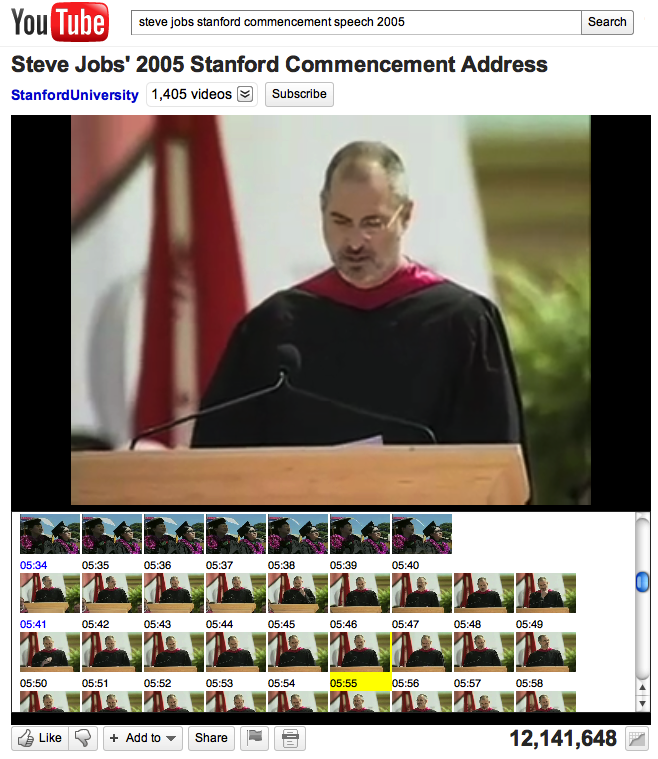
\includegraphics[width=0.95\textwidth,height=0.9\textheight,keepaspectratio]{./stevejobs.png}
  \caption[Camera shots for a~sample video on  
    a~major online video portal]
    {Camera shots for a~sample video on 
    a~major online video portal, detected on-the-fly via
    our shot boundary algorithm incorporated
    in a~browser extension}
  \label{fig:screenshotcamerashots}
\end{figure}

\section{Related Work} 

As outlined before, video fragments consist of shots, which are sequences of
consecutive frames from a~single viewpoint,
representing a~continuous action in time and space.
The topic of shot boundary detection has already been described
extensively in literature.
While some specific issues still remain open
(notably detecting gradual transitions and detected false positives
due to large movement or illumination changes),
the problem is considered resolved for many
cases~\cite{yuan2007shotboundary,hanjalic2002shotboundary}.
Below, we present an overview of several well-known categories of shot boundary detection techniques.

\paragraph{Pixel Comparison Methods:}

Pixel comparison methods~\cite{hampapur1994videosegmentation,
zhang1993videopartitioning} construct a~discontinuity metric
based on differences in color or intensity values
of corresponding pixels in successive frames.
This dependency on spatial location makes this technique
very sensitive to (even global) motion.
Various improvements have been suggested, such as prefiltering
frames~\cite{zhang1995videoparsing},
but pixel-by-pixel comparison methods proved inferior,
which has steered research towards other directions.

\paragraph{Histogram Analysis:}

A~related method to pixel comparison methods is
histogram analysis~\cite{otoole1999shotboundary},
where changes in frame histograms are used
to justify shot boundaries.
Their insensitivity to spatial information
within a~frame makes histograms less prone to partial
and global movements in a~shot.

\paragraph{Hybrid Approaches:}

As a~compromise, a~third group of methods consists of
a~trade-off between the above two
categories~\cite{ahmed1999keyframe}.
Different histograms of several, non-overlapping blocks
are calculated for each frame,
thereby categorizing different regions of the frame
with their own color-based, space-invariant fingerprint.
The results are promising, while computational complexity
is kept to a~minimum, which is why we have chosen
to base our algorithm on a~variation of this approach.

\paragraph{Comparison of Mean and Standard Deviations:}

Other approaches to shot boundary detection include
the comparison of mean and standard deviations
of frame intensities~\cite{lienhart1999comparison}.
Detection using other features such as
edges~\cite{zabih1995scenebreaks} and
motion~\cite{bouthemy1997shotchange} have also been proposed.
However, Gargi \emph{et~al.}\ have shown that
these more complex methods do not necessarily
outperform histogram-based approaches~\cite{gargi2000videoshot}.
A~detailed comparison can be found in
Yuan~\emph{et~al.}\cite{yuan2007shotboundary}.

\section{On-the-fly Shot Boundary Detection Algorithm}
\label{sec:details-of-algo}

As outlined in the previous section,
shot boundary detection is mostly considered a~solved problem
and many efficient approaches exist.
However, to the best of our knowledge,
none of the proposed solutions deals with
the specific issue of detecting camera shots in \emph{streaming} video
in the context of a~Web browser and on-the-fly.
Streaming (HTML5) video has no notion of frames,
but only allows for time-based navigation
via the \texttt{currentTime} attribute.
The algorithm we propose in the sequence of this chapter 
deals effectively with these limitations
and we also show that it works efficiently.

\subsection{Details of the Algorithm}

In this section, we discuss our shot boundary detection algorithm,
which falls in the category of histogram-based algorithms.
Since visually dissimilar video frames
can have similar global histograms,
we take local histograms into account instead. 
We therefore split video frames in freely configurable
rows and columns, \emph{i.e.}, lay a~grid of tiles over each frame.
The user interface that can be seen in \autoref{fig:algorithm}
currently allows for anything from a~$\mathit{1} \times \mathit{1}$ 
grid to a~$\mathit{20} \times \mathit{20}$ grid.
The limits are imposed by the reasonable processing time on consumer PCs.
For each step, we examine a~frame $\mathit{f}$ and its direct
predecessor $\mathit{f - 1}$ and calculate their tile histograms.
We recall that HTML5 streaming video has no notion of frames,
so by frame we mean a~frame that we have navigated to
via setting the \texttt{currentTime} attribute.
Apart from the per-tile average histogram distance,
the frame distance function further considers
a~freely configurable number of \emph{most different} and
\emph{most similar} tiles.
This is driven by the observation that different parts
of a~video have different intensities of color changes,
dependent on the movements from frame to frame.
The idea is thus to boost the influence of movements in the frame
distance function, and to limit the influence of permanence.
In the debug view of our approach that can be seen in
\autoref{fig:algorithm}, blue boxes indicate movements,
while red boxes indicate permanence.
In the concrete example, Steve Jobs' head and shoulders move
as he talks, which can be clearly seen
thanks to the blue boxes in the particular tiles.
Additional movements come from a~swaying flag on the left,
and a~plant on the right.
In contrast, the speaker desk, the white background,
and the upper part of his body remain static,
resulting in red boxes.
We use a~grid layout of $\mathit{20} \times \mathit{20}$ tiles
($\mathit{nTiles} = \mathit{400}$), and
a~$\mathit{tileLimit = 133 = \mathit{20} \times \mathit{20} * 1/3}$
of most different or similar tiles,
\emph{i.e.}, we treat one third of all tiles
as most different tiles, one third as normal tiles,
and one third as most similar tiles,
and apply boosting and limiting factors to the most different
and most similar tiles respectively.
We work with values of~$\mathit{1.1}$ for the
$\mathit{boostingFactor}$, which slightly increases
the impact of the most different tiles,
and $\mathit{0.9}$ for the $\mathit{limitingFactor}$,
which slightly decreases the impact of the most similar tiles.
These algorithm parameters were empirically determined
to deliver solid results on a~large corpus of videos,
albeit for each individual video the optimal settings
can be manually tweaked to take into account the
particular video's special characteristics.
The algorithm pseudocode can be seen in \autoref{code:algorithm}.

We define the average histogram distance between two frames
$\mathit{f}$ and $\mathit{f - 1}$ as $\mathit{avgHisto_{f}}$.
In a~first step, we have examined the histogram distance
data statistically and observed that while
the overall average frame distance $\mathit{avgDist_{f}}$,
defined as $$\mathit{avgDist_{f}} =
\frac{1}{\mathit{nTiles}}\sum_{t=1}^{\mathit{nTiles}}
\mathit{avgHisto_{f, t}}$$ is very intuitive to human beings,
far more value lies in the standard deviation
$\mathit{stdDev_{f}}$, based on the definition of the overall
average frame distance $\mathit{avgDist_{f}}$
$$\mathit{stdDev_{f}} =
\sqrt{\frac{1}{\mathit{nTiles}}\sum_{t=1}^{\mathit{nTiles}}
(\mathit{avgHisto_{f, t}} - \mathit{avgDist_{f}})^{2}}$$
We use the standard deviation as a~value for the shot splitting
threshold~\cite{lienhart1999comparison}
to obtain very accurate shot splitting results.
We found the boosting and limiting factors to have an overall
positive quality impact on more lively videos
and a~negative quality impact on more monotone videos.
Optimal results can be achieved if,
after changing either the boosting or the limiting factors
for the most similar or different tiles,
the value of the shot splitting threshold is adapted
to the new resulting standard deviation.
The user interface can optionally do this automatically.

\begin{figure}
\centering
    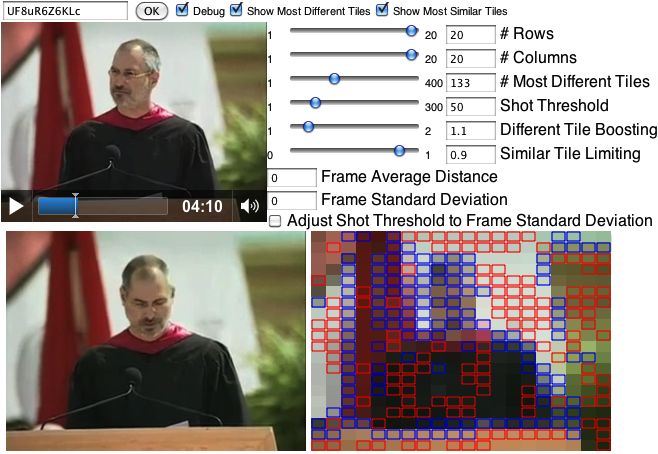
\includegraphics[width=1.0\linewidth]{./algorithm.png}
  \caption[Debug view of the shot boundary detection process]
    {Debug view of the shot boundary detection process.
    Blue boxes highlight tiles with most differences
    to the previous frame, red boxes those with most similarities.}
  \label{fig:algorithm}
\end{figure}

\begin{lstlisting}[caption=Pseudocode of the shot boundary detection
  algorithm,
  label=code:algorithm, float]
for frame in frames
  f = frame.index  
  for tile in tiles of frame      
    avgHisto[f][tile] = getTilewiseDiff()
 
  mostDiffTiles = getMostDiffTiles(avgHisto[f])
  mostSimTiles = getMostSimTiles(avgHisto[f])
 
  for tile in tiles of frame    
    factor = 1  
    if tile in mostDiffTiles
      factor = boostingFactor
    else if tile in mostSimTiles
      factor = limitingFactor
    avgHisto[f][tile] = avgHisto[f][tile] * factor
  avgDist[f] = avg(avgHisto[f])
\end{lstlisting}

\subsection{Implementation Details}
\label{sec:implementation}

The complete video analysis process happens fully
on the client side.
We use the HTML5 JavaScript APIs of the \texttt{<video>} and
\texttt{<canvas>} tags.
In order to obtain a~video still frame
from the \texttt{<video>} tag at the current video position,
we use the \texttt{drawImage()} function of the 2D context of the
\texttt{<canvas>} tag,
which accepts a~video as its first parameter.
We then analyze the video frame's pixels per tile
and calculate the histograms.
In order to retrieve the tile-wise pixel data
from the 2D context of the \texttt{<canvas>},
we use the \texttt{getImageData()} function.
For processing speed reasons, we currently limit our approach to
a~resolution of one second, \emph{i.e.},
for each analysis step,
seek the video in $\mathit{1s}$ steps.
We then calculate the frame distances as outlined in
\autoref{sec:details-of-algo}.
For each frame, we can optionally generate an \texttt{<img>} tag
with a~base64-encoded data URI representation
of the video frame's data
that can serve for filmstrip representations of the video.

We have implemented the shot boundary detection algorithm
as a~stand-alone Web application and as a~browser extension
for the popular video hosting platform YouTube.
Browser extensions are small software programs that users can install
to enrich their browsing experience with their browser.
They are typically written using a~combination of standard Web technologies,
such as HTML, JavaScript, and CSS.
There are several types of extensions; for this work
we focus on extensions based on so-called \emph{content scripts}.
Content scripts are JavaScript programs that run in the context of Web pages
via dynamic code injection.
By using the standard Document Object Model (DOM)~\cite{lehors2004dom},
they can modify details of Web pages.

\section{Evaluation}

On-the-fly shot detection in streaming video
comes with its very own challenges that were briefly outlined before.
First, it is a~question of streaming speed.
Especially with high-definition (HD) video,
this can be very demanding.
We do not attach the analysis \texttt{<video>} and \texttt{canvas} tags
to the DOM tree~\cite{lehors2004dom} so that the browser
does not have to render them and thus can save some CPU cycles,
however, the video playing logic still has to seek the video position
ahead in one-second steps and process the encountered still frame.
Even on a~higher-end computer (our experiments ran on a~MacBook
Pro, Intel Core 2 Duo 2,66 GHz, 8 GB RAM),
the process of in parallel analyzing and displaying
a~$\mathit{1280} \times \mathit{720}$ HD video of media type
\emph{video/mp4; codecs="avc1.64001F, mp4a.40.2"}
caused an average CPU load of about 70\%.
The HTML5~\cite{berjon2012html5} specification states that
\textit{``when the playback rate is not exactly 1.0,
hardware, software, or format limitations can cause video frames
to be dropped''}.
In practice, this causes the analysis environment
to be far from optimal.
In our experiments we differentiated between false positives,
\emph{i.e.}, shot changes that were detected,
but not existent, and misses, \emph{i.e.},
shot changes that were existent,
but not detected.
Compared to a~set of videos with manually annotated shot changes,
our algorithm detected fewer false positives than misses.
The reasons were gradual transitions and shots
shorter than one second (below our detection resolution)
for misses, and large movements in several tiles
for false positives.
Overall, we reached an accuracy of about 86\%,
which is not optimal, but given the challenges
sufficient for our use case of
detecting near- or exact duplicate videos. 

\section{Future Work}

There is potential for optimization of the analysis speed
by dynamically selecting lower quality analysis video files,
given that videos are oftentimes available in several resolutions,
like Standard Definition (SD) or High Definition (HD).
We have checked in how far analysis results differ
for the various qualities,
with the result that SD quality is sufficient.
We have made the shot detection application available online at
\url{http://tomayac.com/youpr0n/} (accessed July 15, 2013) and invite the reader to compare
the results, \emph{e.g.}, the SD video
\url{http://tomayac.com/youpr0n/videos/vsfashionshow_sd.mp4} (accessed July 15, 2013) with
the HD version \url{http://tomayac.com/youpr0n/videos/vsfashionshow_hd.mp4} (accessed July 15, 2013).

Second, more advanced heuristics for the various user-definable
options in the analysis process are possible.
While there is no optimal configuration for all types of videos,
there are some key indicators that can help categorize videos
into classes and propose predefined known working settings
based on the standard deviation $\mathit{stdDev_{f}}$
and the overall average frame distance $\mathit{avgDist_{f}}$.
Both are dependent on the values of $\mathit{boostingFactor}$,
$\mathit{limitingFactor}$, $\mathit{rows}$, and $\mathit{columns}$. 
Interpreting our results, there is evidence
that low complexity settings are sufficient in most cases,
\emph{i.e.}, a~number of $\mathit{rows}$ and $\mathit{columns}$
higher than~$\mathit{2}$ does not necessarily
lead to more accurate shot boundary detection results.
The same applies to the number of to-be-considered most different
or similar tiles $\mathit{tileLimit}$.
We had cases where not treating those tiles differently
at all, \emph{i.e.}, setting
$\mathit{boostingFactor} = \mathit{limitingFactor} = \mathit{1}$, 
led to better results; for example with screencast-type videos,
typically used to demonstrate and teach the use of software features
that were not recorded with a~real camera,
but directly recorded from the computer's screen, with ``camera shots''
then later added with video editing software.

\section{Conclusions}

In this chapter, we have introduced an algorithm for video shot boundary detection
that was implemented as a~stand-alone Web application
and as a~browser extension that adds shot boundary detection to YouTube videos.
While the task of shot boundary detection is considered resolved for many cases,
this is not true for the case of streaming online Web video.
With this research, we have proposed and evaluated an approach
that was shown to deliver consistently good results for all sorts of online videos.
The biggest remaining challenge is finding \emph{the} optimal algorithm settings
for a~given video.
Promising directions for improving the shot boundary detection results
are video categorization (fast-moving, slow-moving, color, black-and-white, \emph{etc.})\ prior
to the actual shot detection process.
By publicly sharing our implementation under a~permissive open-source license,
we open the door for future researchers to build upon our current results.

\section*{Chapter Notes}
This chapter is partly based on the following publications:
\todo{Add publications}

\bibliographystyle{plainnat}
\clearpage
\bibliography{backmatter/references}
